\section{Multi-Chain Deployment Guide}
\label{sec:deployment}

\subsection{Overview}

AI Token launches simultaneously on 10 EVM chains, each with independent 1B supply cap and Bitcoin-aligned mining schedule. This section details the deployment process, LP seeding, and governance setup.

\begin{center}
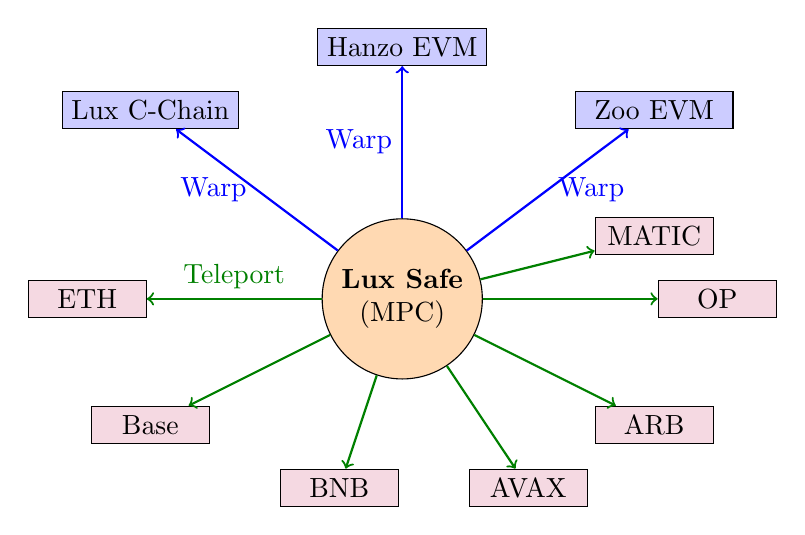
\begin{tikzpicture}[scale=0.8]
    % Central Safe
    \node[draw, circle, fill=orange!30, minimum size=2cm, align=center] (safe) at (0,0) {
        \textbf{Lux Safe}\\(MPC)
    };

    % Lux Native Chains
    \node[draw, rectangle, fill=blue!20, minimum width=2cm] (lux) at (-4,3) {Lux C-Chain};
    \node[draw, rectangle, fill=blue!20, minimum width=2cm] (hanzo) at (0,4) {Hanzo EVM};
    \node[draw, rectangle, fill=blue!20, minimum width=2cm] (zoo) at (4,3) {Zoo EVM};

    % External Chains
    \node[draw, rectangle, fill=purple!15, minimum width=1.5cm] (eth) at (-5,0) {ETH};
    \node[draw, rectangle, fill=purple!15, minimum width=1.5cm] (base) at (-4,-2) {Base};
    \node[draw, rectangle, fill=purple!15, minimum width=1.5cm] (bnb) at (-1,-3) {BNB};
    \node[draw, rectangle, fill=purple!15, minimum width=1.5cm] (avax) at (2,-3) {AVAX};
    \node[draw, rectangle, fill=purple!15, minimum width=1.5cm] (arb) at (4,-2) {ARB};
    \node[draw, rectangle, fill=purple!15, minimum width=1.5cm] (op) at (5,0) {OP};
    \node[draw, rectangle, fill=purple!15, minimum width=1.5cm] (poly) at (4,1) {MATIC};

    % Arrows from Safe
    \draw[->, thick, blue] (safe) -- (lux) node[midway, left] {Warp};
    \draw[->, thick, blue] (safe) -- (hanzo) node[midway, left] {Warp};
    \draw[->, thick, blue] (safe) -- (zoo) node[midway, right] {Warp};
    \draw[->, thick, green!50!black] (safe) -- (eth) node[midway, above] {Teleport};
    \draw[->, thick, green!50!black] (safe) -- (base);
    \draw[->, thick, green!50!black] (safe) -- (bnb);
    \draw[->, thick, green!50!black] (safe) -- (avax);
    \draw[->, thick, green!50!black] (safe) -- (arb);
    \draw[->, thick, green!50!black] (safe) -- (op);
    \draw[->, thick, green!50!black] (safe) -- (poly);
\end{tikzpicture}
\end{center}

\subsection{Deployment Sequence}

\subsubsection{Phase 1: Contract Deployment}

Deploy AIToken contract to all 10 chains using CREATE2 for deterministic addresses:

\begin{lstlisting}[style=solidity]
// Deterministic deployment via CREATE2
bytes32 constant SALT = keccak256("AI_TOKEN_V1_2025");

// Same deployer, same salt = same address on all chains
address aiToken = CREATE2.deploy(
    SALT,
    type(AIToken).creationCode,
    abi.encode(safeAddress, treasuryAddress)
);
\end{lstlisting}

\subsubsection{Deployment Order}

\begin{enumerate}
    \item \textbf{Lux Native Chains (Warp-enabled)}
    \begin{itemize}
        \item Lux C-Chain (96369) - Primary deployment
        \item Hanzo EVM (36963) - AI-focused applications
        \item Zoo EVM (200200) - Research/DeSci applications
    \end{itemize}

    \item \textbf{External EVMs (Teleport-enabled)}
    \begin{itemize}
        \item Ethereum (1) - Largest liquidity
        \item Base (8453) - Coinbase ecosystem
        \item BNB Chain (56) - High transaction volume
        \item Arbitrum (42161) - L2 scaling
        \item Optimism (10) - L2 scaling
        \item Polygon (137) - Low fees
        \item Avalanche (43114) - Fast finality
    \end{itemize}
\end{enumerate}

\subsection{Safe Multi-sig Setup}

\subsubsection{Safe Configuration}

Each chain deployment is managed by a Safe multi-sig wallet:

\begin{center}
\begin{tabular}{lcc}
\toprule
\textbf{Parameter} & \textbf{Lux Native} & \textbf{External} \\
\midrule
Threshold & 3-of-5 & 3-of-5 \\
Key Management & MPC (CGGMP21) & MPC (CGGMP21) \\
Timelock & 24 hours & 48 hours \\
Emergency Pause & 2-of-5 & 2-of-5 \\
\bottomrule
\end{tabular}
\end{center}

\subsubsection{Initial Admin Operations}

\begin{lstlisting}[style=solidity]
// 1. Deploy AIToken
AIToken token = new AIToken(safe, treasury);

// 2. Set genesis block (starts mining schedule)
token.setGenesis();

// 3. Authorize Teleport bridge
token.authorizeBridge(teleportBridge);

// 4. Authorize mining contract
token.authorizeMiner(miningContract);

// 5. Mint LP allocation to seeding address
token.mintLP(lpSeeder, 100_000_000 ether);
\end{lstlisting}

\subsection{LP Seeding Protocol}

\subsubsection{One-Sided LP Strategy}

Each chain receives 100M AI (10\%) for liquidity pool seeding at \$0.10/AI:

\begin{center}
\begin{tabular}{lccc}
\toprule
\textbf{Chain} & \textbf{AI Amount} & \textbf{Target Price} & \textbf{DEX} \\
\midrule
Lux C-Chain & 100M AI & \$0.10 & LuxSwap \\
Hanzo EVM & 100M AI & \$0.10 & HanzoSwap \\
Zoo EVM & 100M AI & \$0.10 & ZooSwap \\
Ethereum & 100M AI & \$0.10 & Uniswap V3 \\
Base & 100M AI & \$0.10 & Aerodrome \\
BNB Chain & 100M AI & \$0.10 & PancakeSwap \\
Arbitrum & 100M AI & \$0.10 & Camelot \\
Optimism & 100M AI & \$0.10 & Velodrome \\
Polygon & 100M AI & \$0.10 & QuickSwap \\
Avalanche & 100M AI & \$0.10 & Trader Joe \\
\bottomrule
\end{tabular}
\end{center}

\subsubsection{LP Pool Creation}

\begin{lstlisting}[style=solidity]
// For Uniswap V2-style DEXs
function createLP(
    address dexRouter,
    address aiToken,
    address nativeToken,
    uint256 aiAmount
) external {
    // 1. Approve router
    IERC20(aiToken).approve(dexRouter, aiAmount);

    // 2. Create pair (AI/NATIVE)
    address pair = IFactory(router.factory()).createPair(
        aiToken,
        nativeToken
    );

    // 3. Add one-sided liquidity (AI only)
    // Initial price set by first swap
    IERC20(aiToken).transfer(pair, aiAmount);
    IPair(pair).sync();
}
\end{lstlisting}

\subsubsection{Initial Price Discovery}

\begin{enumerate}
    \item Safe mints 100M AI to LP seeder contract
    \item LP seeder creates AI/NATIVE pair on DEX
    \item 50M AI deposited as one-sided liquidity
    \item First swap sets price at approximately \$0.10/AI
    \item Market discovery determines actual price
\end{enumerate}

\textbf{Target LP Composition}:
\[
\text{LP Depth} = 50\text{M AI} + \text{Native Token equivalent} \approx \$10\text{M}
\]

At \$0.10/AI:
\[
50\text{M AI} \times \$0.10 = \$5\text{M AI value}
\]

Plus matching native token:
\[
\$5\text{M ETH/BNB/etc} \rightarrow \$10\text{M total depth}
\]

\subsection{Bridge Authorization}

\subsubsection{Lux Native Chains (Warp)}

Warp messaging enables trustless cross-chain communication:

\begin{lstlisting}[style=solidity]
// No additional authorization needed
// Warp is a precompile at 0x0200...0005
// Messages verified by 67% validator quorum
\end{lstlisting}

\subsubsection{External Chains (Teleport)}

Teleport bridge requires explicit authorization:

\begin{lstlisting}[style=solidity]
// On each external chain
token.authorizeBridge(teleportBridgeAddress);

// Teleport bridge configuration
struct TeleportConfig {
    address luxEndpoint;      // Lux T-chain validator set
    uint256 threshold;        // 67-of-100 validators
    address[] validators;     // Active validator set
}
\end{lstlisting}

\subsection{Mining Contract Deployment}

\subsubsection{Mining Contract Setup}

\begin{lstlisting}[style=solidity]
contract AIMiningContract {
    AIToken public immutable aiToken;

    // Per-chain mining configuration
    uint256 public constant BLOCK_REWARD = 79.4 ether;
    uint256 public constant HALVING_INTERVAL = 6_300_000;
    uint256 public constant TREASURY_BPS = 200; // 2%

    // Mining session management
    mapping(bytes32 => Session) public sessions;

    function submitAttestation(
        bytes calldata teeQuote,
        bytes32 sessionId
    ) external {
        // Verify NVTrust TEE quote
        require(verifyTEEQuote(teeQuote), "Invalid attestation");

        // Calculate reward
        uint256 reward = calculateReward(sessionId);

        // Mint via AIToken
        aiToken.mintReward(msg.sender, reward);
    }
}
\end{lstlisting}

\subsubsection{Mining Authorization}

\begin{lstlisting}[style=solidity]
// Safe authorizes mining contract
token.authorizeMiner(miningContractAddress);

// Mining contract can now call mintReward()
\end{lstlisting}

\subsection{Genesis Block Configuration}

\subsubsection{Setting Genesis}

Genesis block marks the start of the mining schedule:

\begin{lstlisting}[style=solidity]
// Called once by Safe after deployment
token.setGenesis();

// After genesis:
// - currentEpoch() returns 0
// - currentReward() returns 79.4 AI
// - Mining can begin
\end{lstlisting}

\subsubsection{Genesis Timing}

\begin{center}
\begin{tabular}{ll}
\toprule
\textbf{Step} & \textbf{Timing} \\
\midrule
Contract deployment & Day 0 \\
Safe configuration & Day 0 \\
Bridge authorization & Day 0-1 \\
LP seeding & Day 1-2 \\
Mining contract deployment & Day 2-3 \\
Genesis block set & Day 3 (coordinated) \\
Mining begins & Day 3+ \\
\bottomrule
\end{tabular}
\end{center}

\subsection{Post-Deployment Verification}

\subsubsection{Verification Checklist}

\begin{enumerate}
    \item \textbf{Contract State}
    \begin{itemize}
        \item[$\square$] \texttt{safe} address correct
        \item[$\square$] \texttt{treasury} address correct
        \item[$\square$] \texttt{genesisBlock} set
        \item[$\square$] Bridge role granted
        \item[$\square$] Miner role granted
    \end{itemize}

    \item \textbf{LP Pools}
    \begin{itemize}
        \item[$\square$] Pair created on DEX
        \item[$\square$] LP tokens locked/burned
        \item[$\square$] Initial price approximately \$0.10
        \item[$\square$] Pool depth approximately \$10M
    \end{itemize}

    \item \textbf{Bridge}
    \begin{itemize}
        \item[$\square$] Teleport endpoints configured
        \item[$\square$] Validator set registered
        \item[$\square$] Test transfer successful
    \end{itemize}
\end{enumerate}

\subsubsection{On-Chain Verification}

\begin{lstlisting}[style=solidity]
// Verify deployment
function verify(address tokenAddress) external view returns (bool) {
    AIToken token = AIToken(tokenAddress);

    // Check constants
    require(token.LP_ALLOCATION() == 100_000_000 ether);
    require(token.MINING_ALLOCATION() == 900_000_000 ether);
    require(token.CHAIN_SUPPLY_CAP() == 1_000_000_000 ether);
    require(token.HALVING_INTERVAL() == 6_300_000);
    require(token.INITIAL_REWARD() == 79.4 ether);

    // Check state
    require(token.genesisBlock() > 0);
    require(token.safe() != address(0));
    require(token.treasury() != address(0));

    return true;
}
\end{lstlisting}

\subsection{Emergency Procedures}

\subsubsection{Pause Operations}

\begin{lstlisting}[style=solidity]
// Emergency pause (2-of-5 threshold)
function emergencyPause() external onlyEmergency {
    _pause();
    emit EmergencyPause(msg.sender, block.timestamp);
}

// Resume requires full Safe approval (3-of-5)
function unpause() external onlyRole(DEFAULT_ADMIN_ROLE) {
    _unpause();
}
\end{lstlisting}

\subsubsection{Bridge Revocation}

\begin{lstlisting}[style=solidity]
// Revoke compromised bridge
token.revokeBridge(compromisedBridge);

// Deploy new bridge with timelock
// 48-hour delay for external chains
timelockController.schedule(
    address(token),
    0,
    abi.encodeCall(token.authorizeBridge, newBridge),
    bytes32(0),
    bytes32(0),
    48 hours
);
\end{lstlisting}

\subsection{Governance Transition}

\subsubsection{Phase 1: Safe Multi-sig (Launch)}

\begin{itemize}
    \item 3-of-5 MPC-managed Safe
    \item Controls all admin functions
    \item 24-48 hour timelock on critical operations
\end{itemize}

\subsubsection{Phase 2: DAO Governance (Month 6+)}

\begin{lstlisting}[style=solidity]
// Transfer admin to DAO
function transferToDAO(address daoGovernor) external onlyRole(DEFAULT_ADMIN_ROLE) {
    // Grant admin to DAO
    _grantRole(DEFAULT_ADMIN_ROLE, daoGovernor);

    // Revoke from Safe (after DAO operational)
    // Safe retains emergency pause only
    _revokeRole(DEFAULT_ADMIN_ROLE, safe);
}
\end{lstlisting}

\subsubsection{Phase 3: Cross-chain Governance (Year 2+)}

\begin{itemize}
    \item AI token voting power across all chains
    \item Votes aggregated via Teleport/Warp
    \item Unified governance for global parameters
    \item Local parameters remain chain-specific
\end{itemize}

\subsection{Deployment Addresses}

\subsubsection{Deterministic Addresses (CREATE2)}

All contracts deployed at same address across chains:

\begin{center}
\begin{tabular}{ll}
\toprule
\textbf{Contract} & \textbf{Address (CREATE2)} \\
\midrule
AIToken & \texttt{0xAI...TOKEN} \\
Mining Contract & \texttt{0xAI...MINE} \\
LP Seeder & \texttt{0xAI...SEED} \\
Teleport Bridge & \texttt{0xAI...BRIDGE} \\
\bottomrule
\end{tabular}
\end{center}

\textit{Note: Actual addresses determined at deployment via CREATE2 with published salt.}

\subsection{Monitoring \& Analytics}

\subsubsection{Key Metrics}

\begin{enumerate}
    \item \textbf{Per-Chain Metrics}
    \begin{itemize}
        \item Total supply minted
        \item LP minted vs remaining
        \item Mining minted vs remaining
        \item Current epoch and reward
        \item Active mining sessions
    \end{itemize}

    \item \textbf{Global Metrics}
    \begin{itemize}
        \item Cross-chain total supply
        \item Teleport volume (24h, 7d, 30d)
        \item Price deviation across chains
        \item Mining hashrate equivalent
    \end{itemize}
\end{enumerate}

\subsubsection{Dashboard Endpoints}

\begin{lstlisting}[style=rust]
// Multi-chain aggregation API
GET /api/v1/ai/stats
{
    "global": {
        "total_supply": "1234567890.00",
        "total_chains": 10,
        "total_miners": 5000,
        "24h_volume": "50000000.00"
    },
    "chains": [
        {
            "chain_id": 96369,
            "name": "Lux C-Chain",
            "supply": "150000000.00",
            "price_usd": "0.12",
            "epoch": 0,
            "reward": "79.4"
        },
        // ... other chains
    ]
}
\end{lstlisting}
